\def\circledarrowRight#1#2#3{ % #1 Style, #2 Center, #3 Radius
    \draw[#1,-latex] (#2) +(50:#3) arc(50:-230:#3);
}
\def\circledarrowLeft#1#2#3{ % #1 Style, #2 Center, #3 Radius
    \draw[#1,latex-] (#2) +(50:#3) arc(50:-230:#3);
}
\begin{figure}[h]
    \centering
    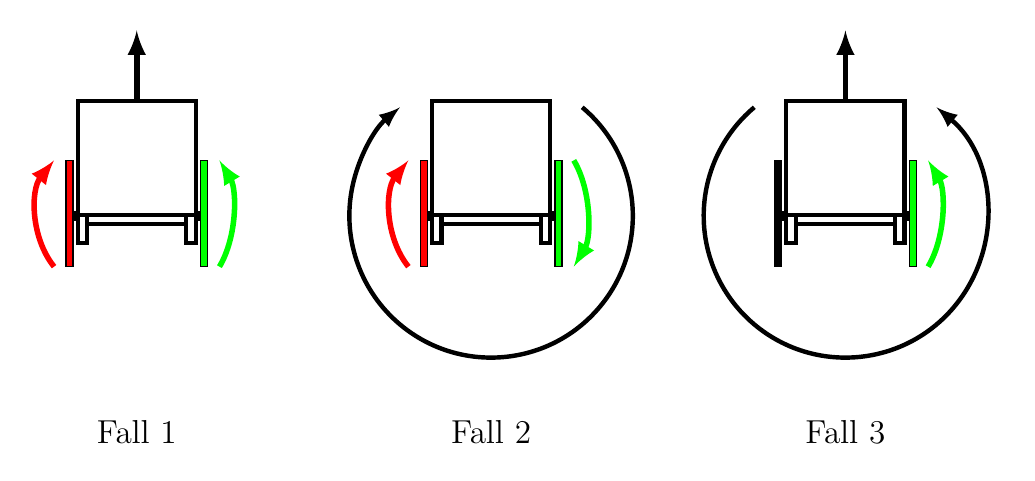
\begin{tikzpicture}[scale=0.3]
        \draw[line width=1, fill=black] (-2.9,0) rectangle (2.9,0.3); %radachse
        \draw[line width=1.5, fill=white] (-2.5,0) rectangle (2.5,5); %sitz
        \draw[line width=1.5, fill=white] (-2.5,-0.2) rectangle (2.5,0.2); %lehne
        \draw[line width=1.5, fill=white] (-2.5,0.2) rectangle (-2.1,-1); %griff links
        \draw[line width=1.5, fill=white] (2.1,0.2) rectangle (2.5,-1); % griff rechts
        \draw[line width=0.5, fill=red] (-3,-2) rectangle (-2.7,2.5); %rad links
        \draw[line width=0.5, fill=green] (2.7,-2) rectangle (3,2.5); %rad rechts
        \draw[-latex, line width=2] (0,5) -- (0,8);
        \draw[-latex, line width=2, color=red] (-3.5,-2) .. controls (-4.5,-0.75) and (-4.5,1.25) .. (-3.5,2.5);
        \draw[-latex, line width=2, color=green] (3.5,-2) .. controls (4.25,-0.75) and (4.25,1.25) .. (3.5,2.5);
        \node [anchor=center, fill=white] at (0,-9) {\large Fall 1};

        % --------------------------------------------------

        % --------------------------------------------------

        \draw[line width=1, fill=black] (12.1,0) rectangle (17.9,0.3); %radachse
        \draw[line width=1.5, fill=white] (12.5,0) rectangle (17.5,5); %sitz
        \draw[line width=1.5, fill=white] (12.5,-0.2) rectangle (17.5,0.2); %lehne
        \draw[line width=1.5, fill=white] (12.5,0.2) rectangle (12.9,-1); %griff links
        \draw[line width=1.5, fill=white] (17.1,0.2) rectangle (17.5,-1); % griff rechts
        \draw[line width=0.5, fill=red] (12,-2) rectangle (12.3,2.5); %rad links
        \draw[line width=0.5, fill=green] (17.7,-2) rectangle (18,2.5); %rad rechts
        \draw[-latex, line width=2, color=red] (11.5,-2) .. controls (10.5,-0.75) and (10.5,1.25) .. (11.5,2.5);
        \draw[latex-, line width=2, color=green] (18.5,-2) .. controls (19.25,-0.75) and (19.25,1.25) .. (18.5,2.5);
        \node (zAxis) at (15,0.15) {};
        \circledarrowRight{ultra thick, black}{zAxis}{6};
        \node [anchor=center, fill=white] at (15,-9) {\large Fall 2};

        % --------------------------------------------------

        \draw[line width=1, fill=black] (27.1,0) rectangle (32.9,0.3); %radachse
        \draw[line width=1.5, fill=white] (27.5,0) rectangle (32.5,5); %sitz
        \draw[line width=1.5, fill=white] (27.5,-0.2) rectangle (32.5,0.2); %lehne
        \draw[line width=1.5, fill=white] (27.5,0.2) rectangle (27.9,-1); %griff links
        \draw[line width=1.5, fill=white] (32.1,0.2) rectangle (32.5,-1); % griff rechts
        \draw[line width=0.5, fill=black] (27,-2) rectangle (27.3,2.5); %rad links
        \draw[line width=0.5, fill=green] (32.7,-2) rectangle (33,2.5); %rad rechts
        \draw[-latex, line width=2] (30,5) -- (30,8);
        \draw[-latex, line width=2, color=green] (33.5,-2) .. controls (34.25,-0.75) and (34.25,1.25) .. (33.5,2.5);
        \node (zAxis) at (30,0.15) {};
        \circledarrowLeft{ultra thick, black}{zAxis}{6};
        \node [anchor=center, fill=white] at (30,-9) {\large Fall 3};
    \end{tikzpicture}
    \caption{Die Bewegungs-Fälle des Rollstuhls aus der Vogelperspektive}
    \label{fig:wheelchairCases}
\end{figure}